\part{Windows Server 2008 R2}
\thispagestyle{plain}
Операционная система \foreignlanguage{english}{Windows Server 2008 R2}, созданная на основе \foreignlanguage{english}{Windows Server 2008}, расширяет базовые возможности операционной системы \foreignlanguage{english}{Windows Server} и предоставляет новые мощные средства, помогая организациям всех размеров повышать управляемость, доступность и гибкость в соответствии с изменяющимися требованиями бизнеса.
Как и Windows 7, Windows Server 2008 R2 использует ядро Windows NT 6.1.
Новые возможности включают улучшенную виртуализацию, новую версию \foreignlanguage{english}{Active Directory Internet Information Services 7.6} и поддержку до 256 процессоров. Система доступна только в 64-разрядном варианте.
\foreignlanguage{english}{Text in language B. This environment switches all language-related definitions, like the language specific names for figures, tables etc. to the other language.}

\section{Получение дистрибутива}
Система \textit{Windows Server 2008 R2} является платным серверным решением корпорации \textit{Microsoft}, получить ознакомительный дистрибутив можно на странице \textit{центра пробного програмного обеспечения TechNet}\footnote{http://technet.microsoft.com/ru-ru/evalcenter/} портала \textit{Microsoft TechNet}.

\section{Выбор выпуска}
\textit{Windows Server 2008 R2} поставляется в нескольких редакциях, приведем сравнительную таблицу версий основанную на ролях сервера:
\begin{figure}[H]
\center{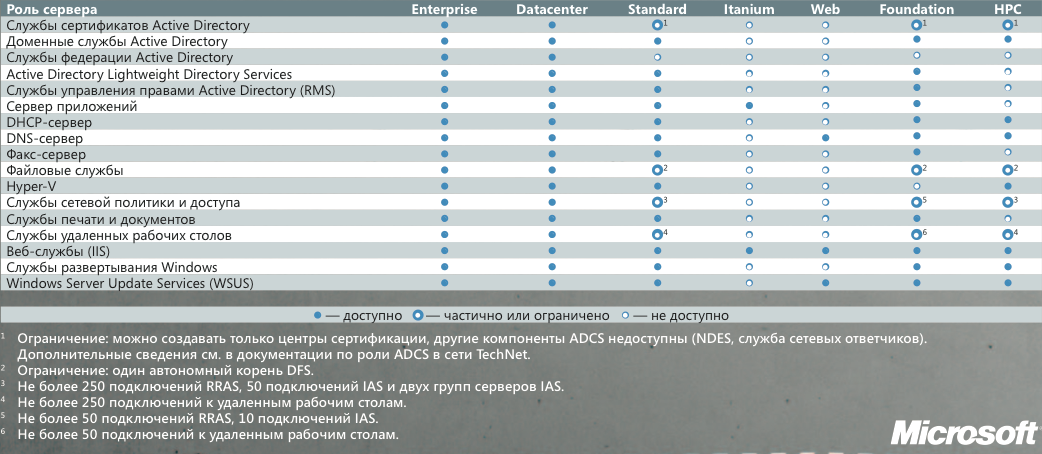
\includegraphics[width=1\linewidth]{ws2k8/diff.png}}
\end{figure}
Как мы видим для наших целей(AD, DNS, DHCP) подойдет выпуск \textit{Standard}.
\newpage
\section{Установка}
Для начала установки загружаемся с установочного диска и настраиваем языковые настройки:
\begin{figure}[H]
\center{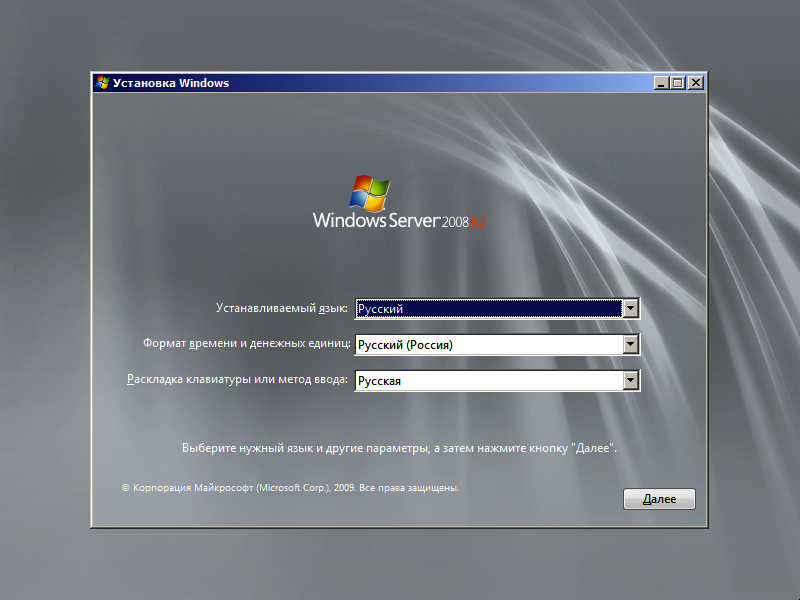
\includegraphics[width=1\linewidth]{ws2k8/install_1.png}}
\caption{Окно языковых настроек}
\label{igas1}
\end{figure}
\clearpage
Для того чтобы приступить к установке, жмем кнопку \textit{Установить}.
\begin{figure}[H]
\center{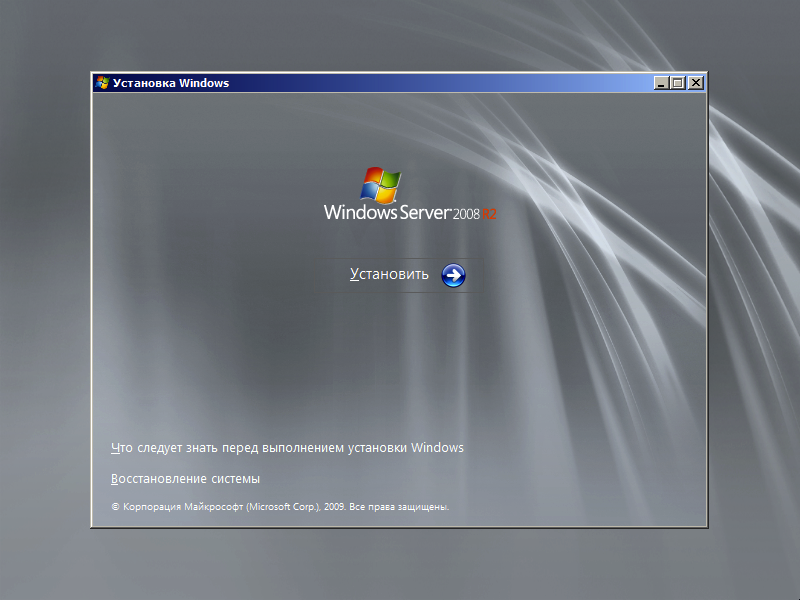
\includegraphics[width=1\linewidth]{ws2k8/install_2.png}}
\caption{Окно начала установки}
\label{igas2}
\end{figure}
\clearpage
Как мы уже решили, мы будем устанавливать версию \textit{Standard} полную, т.к. вариант установки \textit{Server Core} подразумевает минимальную установку и управление из командной строки, этот вариант рассчитан на более опытных пользователей и хуже подходит для обучения.
\begin{figure}[H]
\center{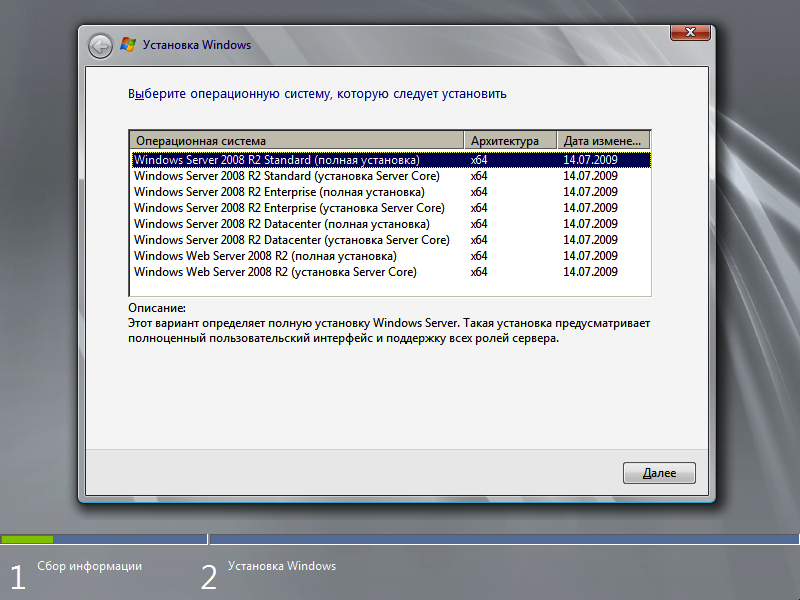
\includegraphics[width=1\linewidth]{ws2k8/install_3.png}}
\caption{Окно выбора редакции}
\label{igas3}
\end{figure}
\clearpage
Ознакомтесь с лицензионным соглашением и если согласны то отметьте соответствующий пункт меню и переходите к следующему шагу.
\begin{figure}[H]
\center{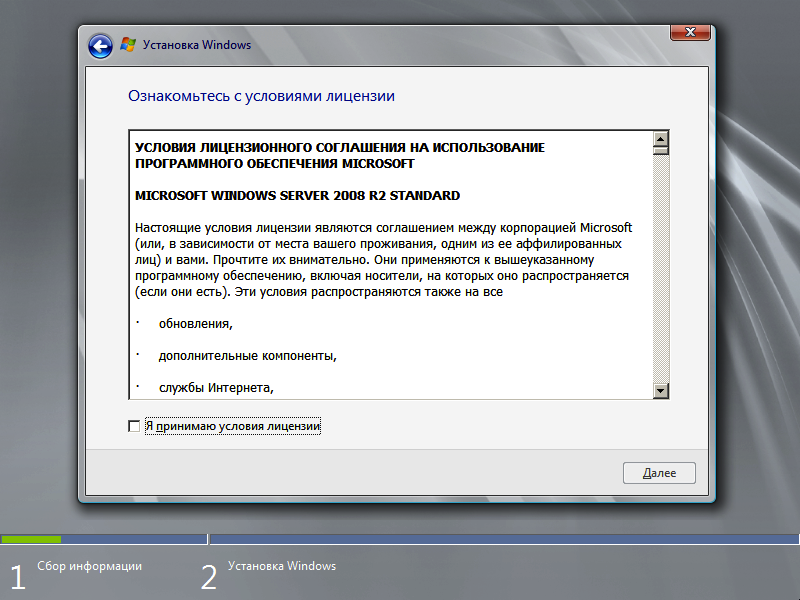
\includegraphics[width=1\linewidth]{ws2k8/install_4.png}}
\caption{Окно лицензионного соглашения}
\label{igas4}
\end{figure}
\clearpage
Выбираем пункт \textit{<<полная установка>>}, т.к. подразумевается что мы настраиваем новый сервер, а обновление существующего сервера выходит за рамки данного пособия.
\begin{figure}[H]
\center{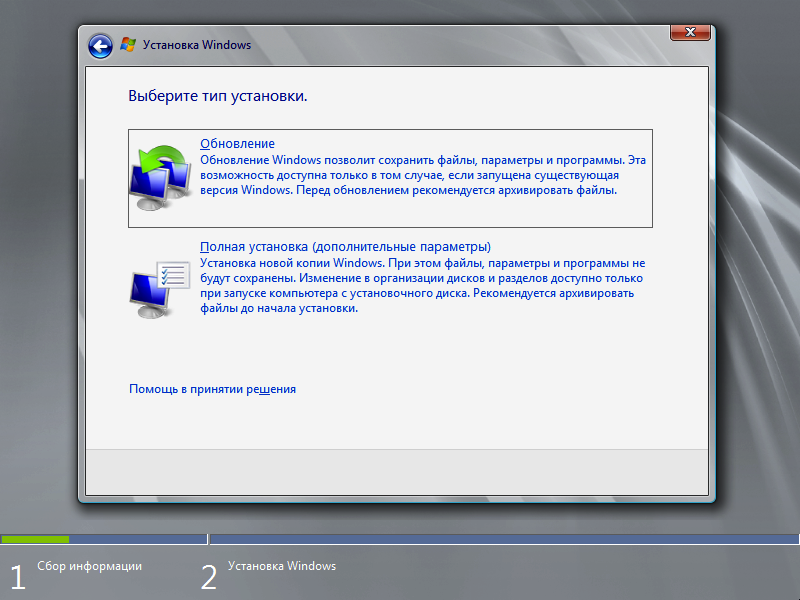
\includegraphics[width=1\linewidth]{ws2k8/install_5.png}}
\caption{Окно способа установки}
\label{igas5}
\end{figure}
\clearpage
У нас не стоит задачи создания резервного копирования данных, поэтому мы можем использовать один локальный диск.
\begin{figure}[H]
\center{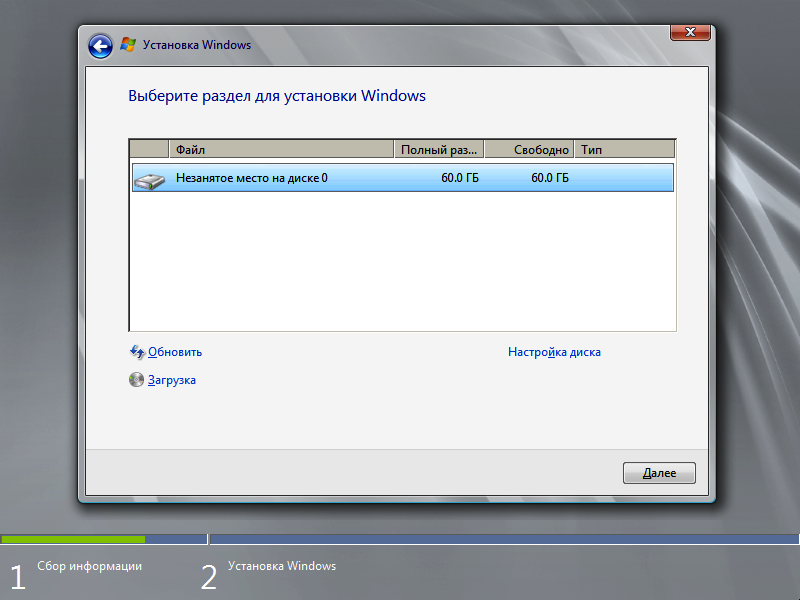
\includegraphics[width=1\linewidth]{ws2k8/install_6.png}}
\caption{Окно разметки диска(ов)}
\label{igas6}
\end{figure}
\clearpage
Ожидаем окончания копирования/распаковки файлов и установки компонентов/обновлений.
\begin{figure}[H]
\center{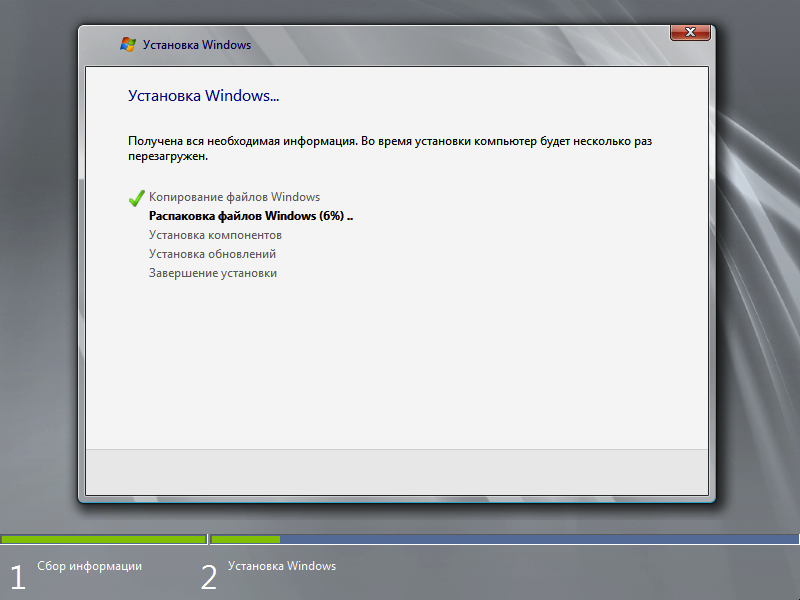
\includegraphics[width=1\linewidth]{ws2k8/install_7.png}}
\caption{Окно установки}
\label{igas7}
\end{figure}
\clearpage
По окончании установки мы увидим окно предупреждения о необходимой перезагрузке.
\begin{figure}[H]
\center{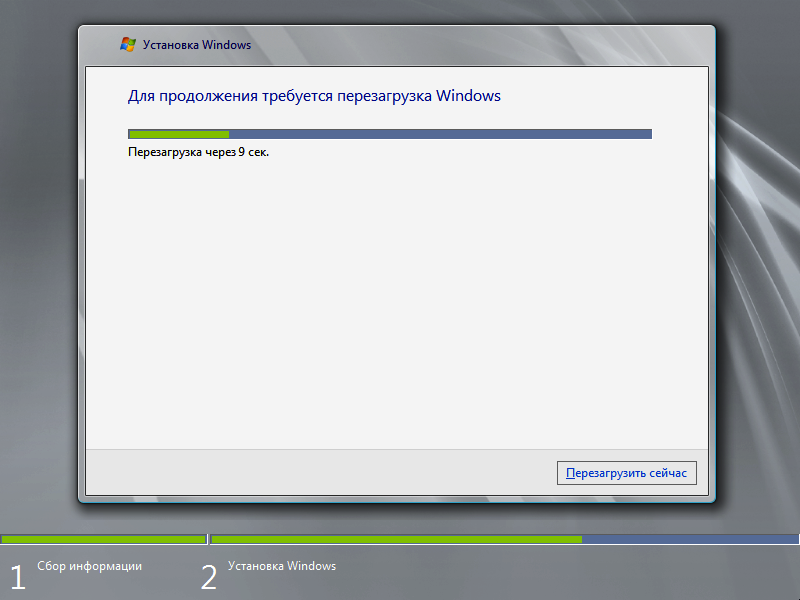
\includegraphics[width=1\linewidth]{ws2k8/install_8.png}}
\caption{Окно перезагрузки}
\label{igas8}
\end{figure}
\clearpage
Завершающий этап установки.
\begin{figure}[H]
\center{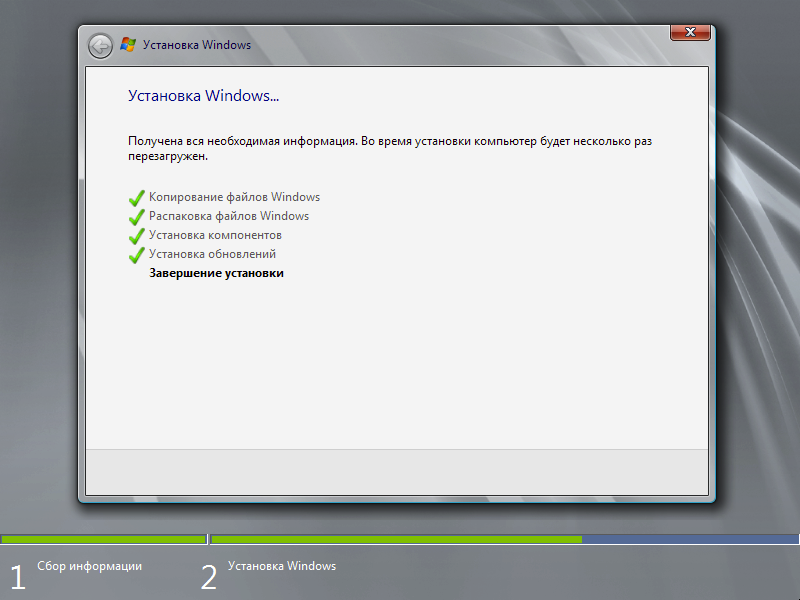
\includegraphics[width=1\linewidth]{ws2k8/install_9.png}}
\caption{Окно завершения установки}
\label{igas9}
\end{figure}
\clearpage
После завершения установки мы увидим предупреждение о необходимости смены пароля администратора.
\begin{figure}[H]
\center{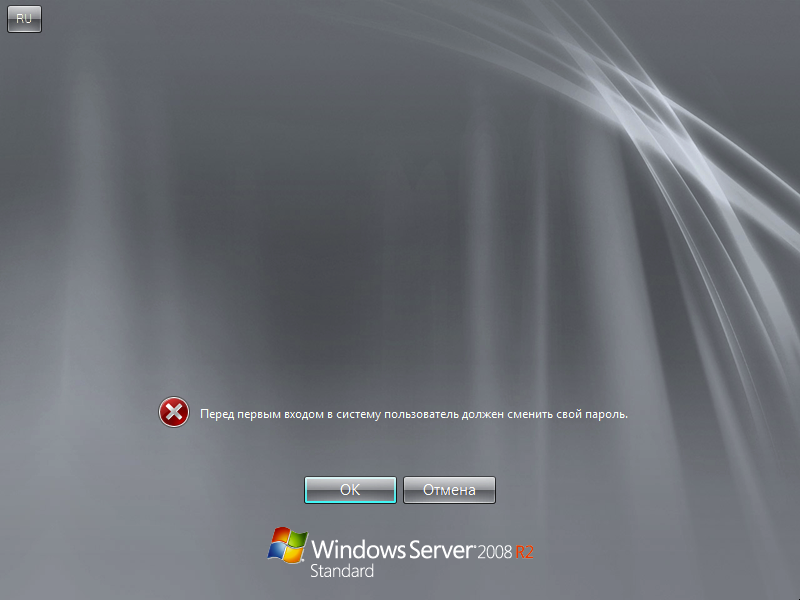
\includegraphics[width=1\linewidth]{ws2k8/install_10.png}}
\caption{Предупреждение}
\label{igas10}
\end{figure}
\clearpage
Последним этапом перед запуском системы является задание пароля для администратора.
\begin{figure}[H]
\center{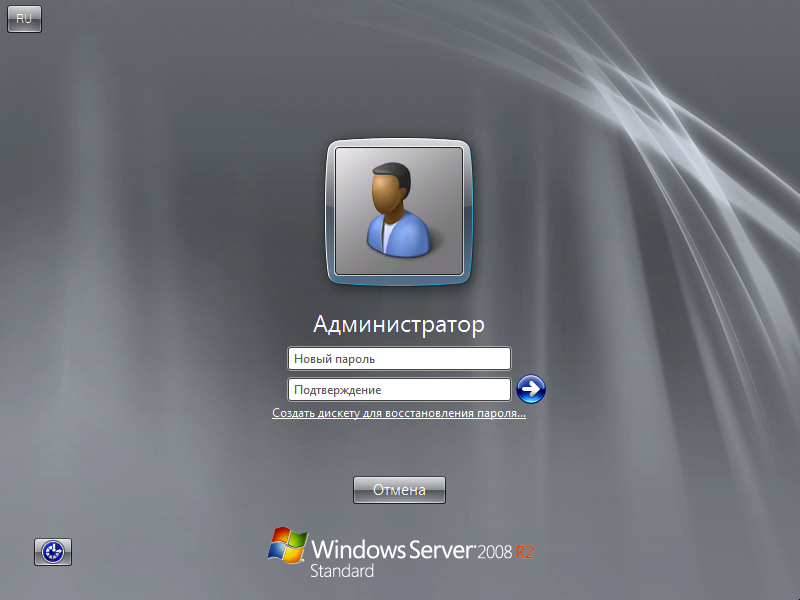
\includegraphics[width=1\linewidth]{ws2k8/install_11.png}}
\caption{Форма смены пароля}
\label{igas11}
\end{figure}

\section{Настройка}
\subsection{Предварительная настройка}
\begin{figure}[H]
\center{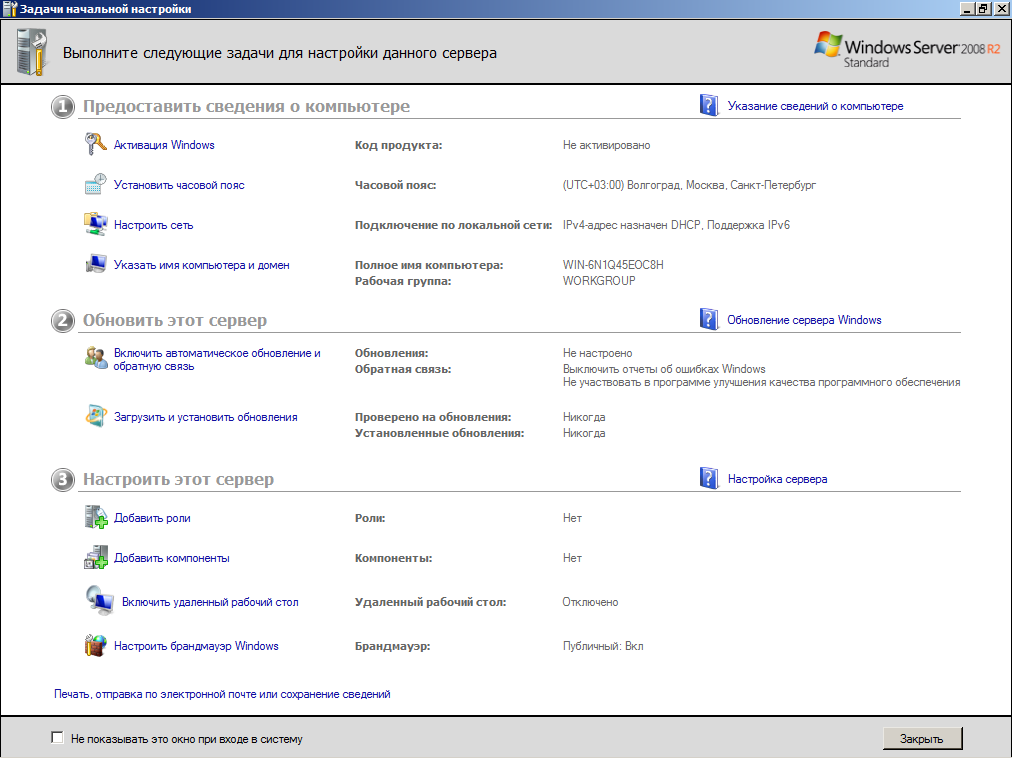
\includegraphics[width=1\linewidth]{ws2k8/setup_1.png}}
\caption{Окно задач начальной настройки}
\label{igas12}
\end{figure}
\newpage
Начнем с настройки сети, перейдем в раздел \textit{Настроить сеть} и зайдем в свойства нашего подключения.
\begin{figure}[H]
\center{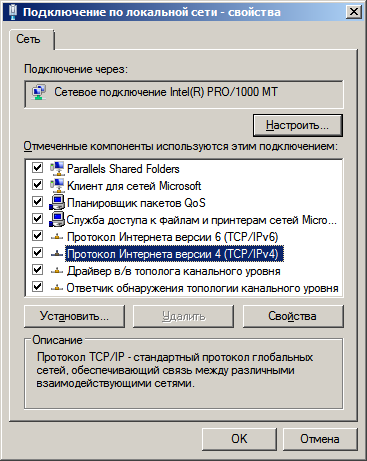
\includegraphics{ws2k8/setup_2.png}}
\caption{Окно задач начальной настройки}
\label{igas13}
\end{figure}
Выберем \textit{Протокол Интернета версии 4 (TCP/IPv4)} и кликнув по кнопке \textit{Cвойства} настроим наше подключение как показанно на рисунке \ref{igas14}.
\begin{figure}[H]
\center{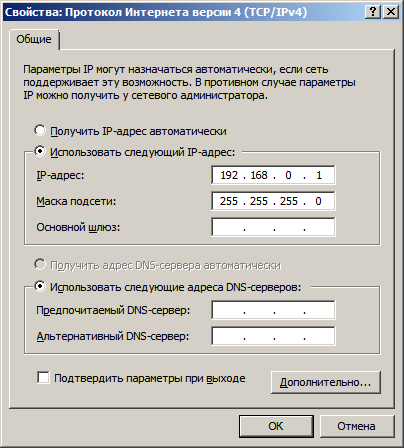
\includegraphics[scale=1]{ws2k8/setup_3.png}}
\caption{Окно задач начальной настройки}
\label{igas14}
\end{figure}
Также следует настроить автоматическое обновление системы, чтобы Ваш сервер был более защищен. Перейдем в раздел \textit{Включить автоматическое обновление и обратную связь}, его можно найти в \textit{Задачах начальной настройки} (рис.~\ref{igas12}). В появившемя окне выбираем \textit{Включить автоматическое обновление Windows и сбор отзывов и предложений}. После этого первоначальную проверку сделаем вручную чтобы не ждать пока это сделает систем по расписанию. Перейдем в раздел \textit{Загрузить и установить обновления} и нажмем на кнопку \textit{Проверка обновлений}, а после как система проверит наличие обновлений нажимаем кнопку \textit{Установить обновления}.
\subsection{DHCP}
Приступим к добавлению первой роли нашего сервера -- DHCP. Из \textit{окна начальной настройки} (\ref{igas12}) в разделе \textit{Настроить этот сервер} нажмем на \textit{Добавить роли}
\subsection{DNS}